\part{Module introduction}
\frame{\partpage}

\begin{frame}{Aim}
\begin{center}
To enable you to apply basic computing and mathematical theory to practical programming activities.
\end{center}
\end{frame}

\begin{frame}{Description}
On this module, you will learn the basic principles of computing, discrete mathematics, and technical notation (e.g. pseudocode, UML, etc.). You start the process of learning to use basic methods and core concepts to solve practical problems and leverage algorithms in your solutions. You will become acquainted in a practical way with the techniques and methods that help you to work effectively and efficiently to build and annotate computing solutions with reference to relevant scholarly sources. You acquire experience of working on basic computing problems and solving them.
\end{frame}

\begin{frame}{Learning Outcomes}
	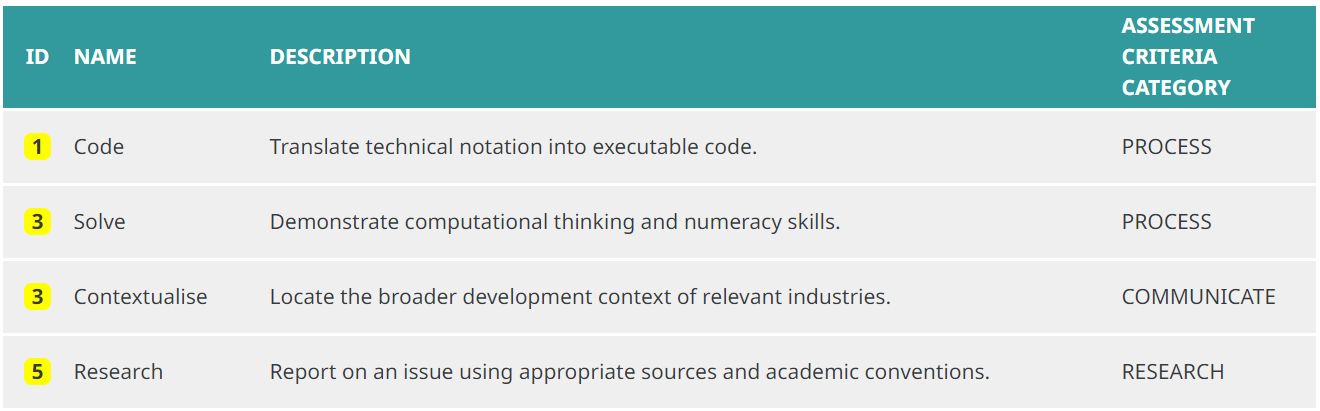
\includegraphics[width=\textwidth]{learning_outcomes}
\end{frame}

\begin{frame}{Module choice}
	\begin{itemize}
		\pause\item If you are on a BSc course (Computing for Games or Immersive Computing) this module is \textbf{mandatory}
		\pause\item If you are on BA Game Development: Programming, this module is \textbf{optional} and can be switched with GAM120: Reading Experiences
		\pause\item Undecided? The induction session for GAM120 is Tuesday 12:00 in DM Lecture A
		\pause\item Want to switch? See me or Michael
	\end{itemize}
\end{frame}

\begin{frame}{Topic schedule}
	\begin{center}
		On LearningSpace
	\end{center}
\end{frame}

\begin{frame}{Timetable}
	\begin{center}
		\url{http://mytimetable.falmouth.ac.uk}
	\end{center}
\end{frame}

\begin{frame}{Assignments}
	\begin{itemize}
		\pause\item Assignment 1: worksheet tasks
			\begin{itemize}
				\pause\item \textbf{Nine} worksheets --- programming, annotation, problem solving, mathematics
			\end{itemize}
		\pause\item Assignment 2: research journal
		\pause\item See LearningSpace for assignment briefs and worksheets
		\pause\item See MyFalmouth for deadlines
	\end{itemize}
\end{frame}

\begin{frame}{Worksheet A}
	\begin{itemize}
		\item SpaceChem
		\item Due \textbf{next Friday (4th October)}
	\end{itemize}
\end{frame}
